\chapter{Introdução}
\label{chap:introduction}

Este relatório pretende demonstrar o trabalho realizado para este projeto.
O mesmo consiste num mecanismo de controlo de portas TCP/UDP \cite{rfc9293},
\cite{rfc768} dos \textit{containers} ou do próprio sistema \textit{host}
da plataforma Forge do IPMAIA.

Esta extensão à plataforma Forge, tem 
como principal objetivo de facilitar a gestão as conexões \textit{containers} 
que são disponibilizados, fazendo uso de ima interface \textit{web}, onde o adminitrador da 
plataforma pode receber pedidos para abrir novas conexões. 

Para a concretização deste trabalho são necessários os seguintes objetivos:\\

\begin{itemize}
\item \textit{Daemon} que irá interagir com a \textit{firewall} ou \acrshort{api}\footnote{\acrshort{api} -- \acrlong{api}} do sistema de \textit{containers};
\item Interface \textit{Web} e \acrshort{api} para interagir com o Daemon;
\item Sistema de notificações de eventos para Microsoft Teams, Discord e E-mail.
\end{itemize}


\section{Objetivos}
\label{sec:object}

Pretende-se, com este projecto, acrescentar funcionalidades/facilitar tarefas na plataforma ao
DevLab/Forge do IPMAIA/UMAIA que permitam:

\begin{itemize}
\item o administrador do sistema facilmente defenir regras de \textit{firewall} no sistema host da plataforma (através do terminal ou de uma interface web);
\item a atribuíção de endereços \acrshort{ip}\footnote{\acrshort{ip} -- \acrlong{ip}} a \textit{containers} hospedados na plataforma, de modo,
a dar conectividade aos mesmos (através do terminal ou de uma interface web);
\item controlar quais portas dos \textit{containers} são disponiibilizadas para a rede interna da intituição;
\item os alunos, aos quais, lhes foram atribuídos um \textit{container}, fazer um pedido ao administrador do sistema para poder
obter ou não conectividade em determinada porta \acrshort{tcp}/\acrshort{udp};
\item os alunos que efetuaram um pedido de abertura de porta, receber notificação (por Microsoft Teams, Discord ou E-mail) quando O
pedido for aceite ou negado.

\end{itemize}

Com a enumeração dos objetivos referidos, serão demonstrados ao longo deste documento
todo o proceso de desnvolvimentos dos mesmos.




\section{Metodologia}
\label{sec:intro_method}

A metodologia usada neste projeto começa com o desenvolvimento base do "Port Controller",
da Rest API e da unix socket que permite aos dois comunicarem. Após ter essa base funcional
foi realizada uma pesquisa sobre Iptables, Nftables, LXC e LXD e de como interagir estes, tanto
por linha de comandos como através de código C\#. Foi feita também uma pesquisa de como
outras plataformas abordam o tópico de controlo de conexões de \textit{containers}.
Por consequente, deu-se continuidade ao desenvolvimento do "Port Controller" e dos 
restantes componentes e à realização de testes dos mesmos.


\section{Recursos tecnológicos}
\label{sec:intro_resources}


No que diz respeito a recursos tecnológicos, optou-se por usar as seguintes opções:

\begin{itemize}
\item Linguagem C\# com o \textit{framework .NET Core} 7.0 para a criacção do \textit{daemon} que gere
as portas dos \textit{containers} e \textit{unix socket de servidor};
\item Linguagem Python versão 3.11 a \textit{unix socket} cliente;
\item Linguagem Python versão 3.11 com a biblioteca Flask para a API e sistemas de notificações;
\item Linguagem Python versão 3.11 com a biblioteca Flask interface \textit{Web}, juntamente com \acrshort{html}\footnote{\acrshort{html} -- \acrlong{html}}, \acrshort{css}\footnote{\acrshort{css} -- \acrlong{css}}, Javascipt e Bootstrap.
\item Máquina virtual com alpine linux 3.19 e \acrshort{wsl}\footnote{\acrshort{wsl} -- \acrlong{wsl}} com ubuntu 22.04 para testar o projeto.
\end{itemize}




\section{Cronograma}
\label{sec:intro_chronos}

\begin{figure}[H]
\begin{center}
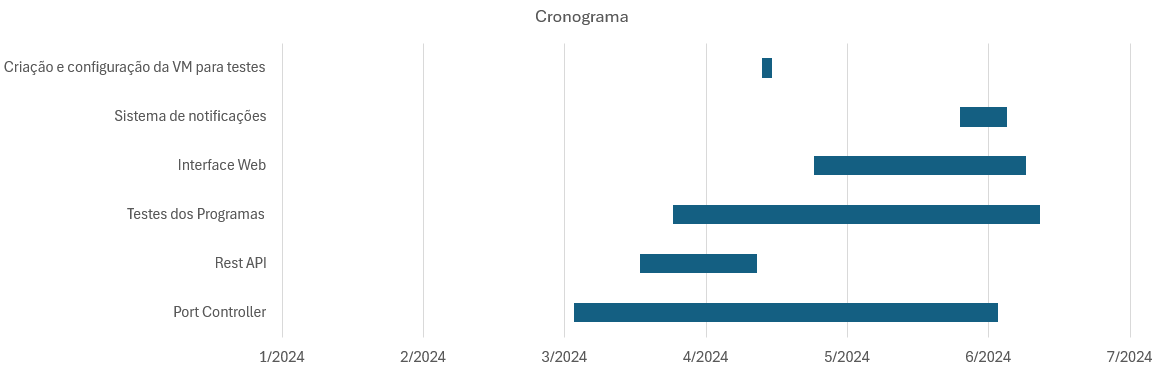
\includegraphics[width=16cm]{figs/cronograma.png}
\caption{Cronograma do projeto}
\label{fig:bookstack}
\end{center}
\end{figure}


\section{Organização do relatório}
\label{sec:intro_struct}

Este documento está organizado pelos seguintes tópicos:

Este relatório está organizado e vários capítulos, de modo, a explicar de forma
eficaz todo o processo no decorrer da elaboração deste projeto.

O documento inicia-se com o Resumo em língua Portuguesa e o Resumo em língua 
inglesa (Abstract), seguindo-se a Declaração de honra e dos Agradecimentos.

O capítulo 1, Introdução, apresenta o tema do projeto realizado, mencionado tópicos
como os Objetivos e Recursos tecnológicos.

No capítulo 2, Análise do problema, é explicado os problemas que este projeto 
pretende resolver.

No capítulo 3, Fundamentos teóricos, são referidos tecnologias e conceitos relevantes 
para o desenvolvimento do projeto, nela são mencionadas as linguagens de programação usadas,
programas utilizados e funcionamento destes.

O capítulo 4, Estado da Arte, dá exemplos do funcionamento das conexões de outras 
plataformas, tais como Google Cloud e Microsoft Azure.

No capítulo 5, Desenvolvimento do tema, onde é abordado as configurações do sistema
de testes, testes do iptables e LXD e desenvolvimento do código dos componentes 
do projeto.


No capítulo 6, Desvios de procedimento, fala sobre pontos que se desviaram do planeamento inicial.

Segue-se o capítulo 7, para apresentar a Discussão de resultados.

No capítulo 8, Trabalho futuro, são referidas possiveis melhoramentos ou adição de funcionalidades
do projeto.

Por fim, no capítulo 9, apresenta-se as Conclusões e a reflexão crítica.


\section*{Sumário}
\label{sec:intro_summary}
%Se considerar relevante, faça um pequeno resumo do capítulo. É uma secção opcional que pode ser eliminada, mas altamente recomendada.
Considera-se assim haver uma possibilidade de aumentar a segurança e controlo do que é disponibilizado
pelos \textit{containers} atribuídos aos alunos.
\\
\\
%Abaixo deve usar a instrução {\textbackslash}cite\{\} para colocar uma relação das citações utilizadas no texto deste capítulo. Aqui liste apenas as citações, pela ordem em que aparecem no texto -- não coloque mais texto. Exemplo:
\\
\\
%\textbf{Referências relevantes:}  \cite{ismai_ead}, \cite{rfc4512}.